\documentclass[journal]{IEEEtran}
% IEEE Transactions on Industrial Informatics -- anonymous regular-paper draft
% Compile: latexmk -pdf main.tex
\usepackage{amsmath,amssymb,amsfonts}
\usepackage{algpseudocode}
% Local XeTeX/Tectonic builds: route IEEEtran's ptm (Times) family requests to
% the legacy Times Type1 faces so metrics match the pdfLaTeX reference build;
% the latexmk -pdf (pdfLaTeX) path is unaffected.
\usepackage{iftex}
\ifxetex
  \DeclareFontFamily{TU}{ptm}{}
  \DeclareFontShape{TU}{ptm}{m}{n}{<->ptmr8t}{}
  \DeclareFontShape{TU}{ptm}{b}{n}{<->ptmb8t}{}
  \DeclareFontShape{TU}{ptm}{m}{it}{<->ptmri8t}{}
  \DeclareFontShape{TU}{ptm}{b}{it}{<->ptmbi8t}{}
  \DeclareFontShape{TU}{ptm}{m}{sl}{<->ptmro8t}{}
  \DeclareFontShape{TU}{ptm}{m}{sc}{<->ptmr8t}{}
\fi
\usepackage{graphicx}
\usepackage{booktabs}
\usepackage{tabularx}
\usepackage{array}
\usepackage[table]{xcolor}
\usepackage{stfloats}
\usepackage{placeins}
\usepackage{url}
\urlstyle{same}
% Cross-references and citations. The cite package renders IEEE-style citation
% groups ([14]--[16], [20], [21]) with hyperref support.
\usepackage{cite}
\usepackage[colorlinks=true,linkcolor=black,citecolor=black,urlcolor=black]{hyperref}
\hypersetup{bookmarksnumbered=true,
  pdftitle={AgentWorkShop: A Reference Implementation for Task-to-Device Integration in Industrial Agents},
  pdfauthor={},
  pdfsubject={IEEE Transactions on Industrial Informatics},
  pdfkeywords={industrial informatics, industrial agents, multi-agent systems, production system integration, semantic data integration}}

% Float placement only; IEEEtran margins and body type remain unchanged.
\setcounter{topnumber}{4}
\setcounter{bottomnumber}{3}
\setcounter{totalnumber}{7}
\setcounter{dbltopnumber}{2}
\renewcommand{\topfraction}{0.95}
\renewcommand{\bottomfraction}{0.80}
\renewcommand{\textfraction}{0.03}
\renewcommand{\floatpagefraction}{0.72}
\renewcommand{\dbltopfraction}{0.95}
\renewcommand{\dblfloatpagefraction}{0.72}

% Tight but conventional float separation; body type and margins are unchanged.
\setlength{\textfloatsep}{8pt plus 2pt minus 3pt}
\setlength{\dbltextfloatsep}{8pt plus 2pt minus 3pt}
\setlength{\intextsep}{7pt plus 2pt minus 3pt}
\setlength{\abovecaptionskip}{3pt plus 1pt minus 1pt}
\setlength{\belowcaptionskip}{2pt plus 1pt minus 1pt}

% Evidence snapshot: one archived integrated run with raw reports, run
% manifest, scenario definitions, and metrics.
% The two live engine-task logs are original outputs saved at execution time,
% as confirmed by the author; the structured run report retains their checked
% outcomes. The four-arm ablation has its own companion run record.
\newcommand{\resSeed}{42}
\newcommand{\resPhases}{20}
\newcommand{\resChecksTotal}{83}
\newcommand{\resChecksPass}{83}
\newcommand{\resChecksWarn}{0}
\newcommand{\resChecksFail}{0}
\newcommand{\resTotalWall}{26\,min}
\newcommand{\resDaqSamples}{55}
\newcommand{\resWriteP}{29.954\,ms}
\newcommand{\resTcpP}{47.8\,ms}
\newcommand{\resOpcP}{19.8\,ms}
\newcommand{\resMqttP}{19.3\,ms}
\newcommand{\resHttpP}{32.9\,ms}
% p95 per protocol line, same run: ~6 writes each. Recorded in the archive's
% metrics.csv (write_p95_ms) but reported in the body only since the 2026-10-12
% revision, so they live here rather than inline. Names must be letters only:
% \resTcpP95 would parse as \resTcpP followed by the characters "95".
\newcommand{\resTcpTail}{248.9\,ms}
\newcommand{\resOpcTail}{20.5\,ms}
\newcommand{\resMqttTail}{20.1\,ms}
\newcommand{\resHttpTail}{44.6\,ms}
% cross-protocol ranges over the four write families (min p50 = MQTT, max
% p50 = Modbus TCP; min p95 = MQTT, max p95 = Modbus TCP)
\newcommand{\resPfiftyRange}{19.3--47.8\,ms}
\newcommand{\resPninetyfiveRange}{20.1--248.9\,ms}
\newcommand{\resWriteNperLine}{6}
\newcommand{\resAblationRun}{\texttt{20260921181234-e1lite}}
\newcommand{\resFullIntercept}{18/18}
\newcommand{\resNoInterlockIntercept}{12/18}
\newcommand{\resNoReadbackIntercept}{18/18}
\newcommand{\resUngatedIntercept}{12/18}
\newcommand{\resBackstop}{130.2\,s}
% 134.7 s: defined but NOT used in the body (the drill's archived timing is
% 130.196 s, = \resBackstop); kept only so the symbol is not silently reused.
\newcommand{\resBackstopDrill}{134.7\,s}
\newcommand{\resPortFfive}{9/9}
\newcommand{\resPortCode}{0}
\newcommand{\resParamChecks}{4/4}
\newcommand{\resHitlLatency}{461\,ms}
\newcommand{\resMissionFrom}{200}
\newcommand{\resMissionTo}{204.704}
\newcommand{\resMissionPv}{204.70}
\newcommand{\resMissionTarget}{$204.704\pm0.75$}
\newcommand{\resBiaxSp}{30}
\newcommand{\resBiaxDaq}{19}
\newcommand{\resBiaxWrites}{3}
\newcommand{\resBiaxStart}{28.10}
\newcommand{\resBiaxFinal}{25.66}
\newcommand{\resBiaxTarget}{25.0}
\newcommand{\resBiaxTol}{0.7}
\newcommand{\resLlmWall}{156.3\,s}
\newcommand{\resGoalWall}{637.3\,s}
\newcommand{\resGoalFinal}{51.7}
\newcommand{\resJstar}{89.894}
\newcommand{\resJzero}{67.2}
\newcommand{\resControllerMin}{0.965}
\newcommand{\resControllerMean}{0.969}
\newcommand{\resControllerMax}{0.972}
\newcommand{\resInjStart}{31.25}
\newcommand{\resInjFinal}{32.17}
\newcommand{\resInjWrites}{2}
\newcommand{\resInjWall}{26.48\,s}
\newcommand{\resWwtpStart}{0.21}
\newcommand{\resWwtpFinal}{3.50}
\newcommand{\resWwtpWrites}{15}
\newcommand{\resWwtpWall}{169.27\,s}
\newcommand{\resWwtpCostStart}{181.5}
\newcommand{\resWwtpCostFinal}{179.1}
\newcommand{\resAnnealStart}{134.52}
\newcommand{\resAnnealFinal}{100.08}
\newcommand{\resAnnealWrites}{5}
\newcommand{\resAnnealWall}{102.76\,s}
\newcommand{\resAnnealSpeedFinal}{164}
\newcommand{\resAnnealSpeedTried}{176}
\newcommand{\resAnnealGain}{17.1\%}
% writeLockSeconds: node field default 30 s, constructor default 60 s; the
% online path enforces max(60 s, configured), so 60 s is the effective floor
% (unused in body since the pacing-window rewrite; kept for reference).
\newcommand{\resWriteLock}{60\,s}

% October 2026 deployment-scale campaign (v0.7.57), added with the revision.
% The hardened-pipeline run is archived at 91/91; three consecutive
% full-suite runs score 79/79 each (237 total; an earlier 80-per-run tally
% counted one S7 report assertion that is not a logged check). Per-run
% reports, manifests, and timelines are archived with each benchmark run.
\newcommand{\resPipeRun}{\texttt{benchmark-20261008045434}}
\newcommand{\resPipeTotal}{91}
\newcommand{\resPipeApi}{54}
\newcommand{\resCampaignRuns}{three consecutive}
\newcommand{\resCampaignTotal}{237}
\newcommand{\resCampaignApi}{45}
\newcommand{\resLoopTotal}{53}
\newcommand{\resAckTotal}{34}
\newcommand{\resDocsTotal}{91}
\newcommand{\resLinesLive}{34}
\newcommand{\resLinesRunning}{17}
% channel count across the three October 9 regression runs: 111/111/113;
% the body reports the range rather than one run's value.
\newcommand{\resChannelsLive}{111--113}
\newcommand{\resDaqOnline}{67}
\newcommand{\resWriteNodesLive}{77}
\newcommand{\resRecipesLive}{52}
\newcommand{\resBindingsLive}{385}
% approval->dispatch spans both campaigns: 8/9/9 ms (Oct 7-8), 9/6/6 ms (Oct 9).
\newcommand{\resHitlDispatchMs}{6--9\,ms}
\newcommand{\resLadderFrom}{66}
\newcommand{\resLadderTo}{63}
\newcommand{\resConsistencyErr}{0.0\,bar}
\newcommand{\resObsVerifyFast}{25.1\,s}
% 245.204 s (benchmark-20261007194413) / 245.184 s (-07194925), exact values
\newcommand{\resObsVerifyCadence}{245.20/245.18\,s}
\newcommand{\resCadenceWait}{218\,s}
\newcommand{\resWideRows}{869}

% October 9, 2026 regression campaign (v0.7.57), same live instance.
% Three runs archived at 92/92, 90/90, and 90/90; timeline.jsonl per run
% (S4/S5 process records, HITL card events).
\newcommand{\resNovRuns}{\texttt{benchmark-20261009021149}/\texttt{-024141}/\texttt{-033810}}
\newcommand{\resNovTotal}{272}
\newcommand{\resNovApi}{54}
\newcommand{\resNovDeadband}{0.15\,g}
\newcommand{\resNovZigzagFrom}{64}
\newcommand{\resNovZigzagTo}{63}
\newcommand{\resNovCorrFrom}{63}
\newcommand{\resNovCorrTo}{65}
\newcommand{\resNovWeights}{$32.49/32.33/32.22$\,g}
\newcommand{\resNovCadenceReject}{69\,s}
\newcommand{\resNovCardId}{\texttt{ap-2950a5b6}}
\newcommand{\resNovRunId}{\texttt{rr-51b0a0ac}}
\newcommand{\resNovScheme}{hold-pressure micro-up (sensitivity excitation step)}
\newcommand{\resNovSlope}{0.052\,g/bar}
% Oct 9 diagnostics: three-run distribution, not the single worst run.
% runs 021149/024141/033810: rows 663/843/861, in-spec 100.0/96.4/94.0%,
% std 0.042/0.186/0.237 g. \resNovInspec/\resNovWideRows/\resNovStd are the
% single third-run values; the ranges above are defined for reference and
% \resRowsRange is the one used in the body.
\newcommand{\resNovInspecRange}{94.0--100.0\%}
\newcommand{\resNovStdRange}{0.04--0.24\,g}
\newcommand{\resRowsRange}{663--869}
\newcommand{\resNovInspec}{94.0\%}
\newcommand{\resNovWideRows}{861}
\newcommand{\resNovStd}{0.24\,g}

% Seven-leg fault-suite outcomes (hardening ack-gate suite,
% tmp-e2e/hardening-ack-gate.mjs; archived in
% docs/audit/2026-10-08-production-hardening-report.md): 2 parameters
% promoted transport-acknowledged -> readback-verified by post-write
% re-read; 1 failed (broker unreachable, healthy sibling verified);
% 1 unverified (publish-only endpoint, three verification attempts).
\newcommand{\resAckPromoted}{2}
\newcommand{\resAckFailed}{1}
\newcommand{\resAckUnverified}{1}


\newcommand{\system}{the platform}

\begin{document}
\bstctlcite{IEEEbstctl}

\title{AgentWorkShop: A Reference Implementation for Task-to-Device Integration in Industrial Agents}

\author{}
\markboth{IEEE Transactions on Industrial Informatics, Submitted Manuscript}{AgentWorkShop: Task-to-Device Integration}

\maketitle

\begin{abstract}
Industrial agents need a software path that connects a task to production
context, semantic operations, and configured device interfaces. AgentWorkShop
is a modular reference implementation that composes task services, registered
harnesses, line--product--recipe--run context, per-call operation checks,
semantic I/O, protocol drivers, and service-owned records. It resolves context
for each agent turn and checks applicable authority at dispatch; prompt
context grounds a proposal but is not a task-pinned authorization token. We
evaluated one registered harness in cast-film and annealing simulators with
different signal and protocol mappings. Six sequential tasks completed with
synthetic approval and verified device readback, and all six records passed
task-to-approval, receipt, and active-run sample linkage checks. All six
samples remained outside their target bands. The result demonstrates the
tested record path, not process attainment or cross-harness portability.
\end{abstract}

\begin{IEEEkeywords}
Industrial agents, industrial communication, industrial informatics,
production systems, semantic data integration.
\end{IEEEkeywords}

\IEEEpeerreviewmaketitle

\section{Introduction}
\IEEEPARstart{I}{ndustrial-agent} deployments must connect each task to its
production context, process signals, and equipment interfaces. Existing work
addresses end-to-end automation control, operator-reviewed control-sequence
generation, modular factory skills, and production scheduling
\cite{xia2025control,huang2026made,koehle2026llmdriven,waseem2026pretrained}.
Other studies target PLC code generation, context-aware control, resource
capability discovery, shop-floor coordination, digital-twin fault handling,
natural-language machine access, and robotic-line control
\cite{liu2026agents4plc,wu2025instructmpc,lim2025llmenabled,zhao2026shopfloor,gill2025llmdt,hofmann2025nlc}.
Across production lines, agent roles, signal maps, protocols, objectives, and
product/run context vary. An integration architecture must accommodate these
differences around shared task and operation services while keeping each
action tied to its active production context.

Consider two production scenes with different process signals and interfaces:
cast-film thickness control and annealing-zone temperature control. An agent
task in either scene needs production context, typed signal access, and a
route from a named operation to the configured device protocol. The framework
must also distinguish a command receipt from a subsequent process
observation. The shared task and operation services can therefore be
configured with scene-specific signal maps, protocols, and limits while
retaining a common execution path. The evaluation instantiates this path in
two simulator scenes.

This paper presents AgentWorkShop as a reference implementation of
task-to-device integration for industrial agents. It connects collaborative tasks
and registered harnesses to production context, manufacturing execution
system (MES) data, analysis and modeling services, data-acquisition (DAQ) and
write-control (DCW) nodes, and protocol-specific drivers. Its interfaces include
command-line, web, SDK, REST, Model Context Protocol (MCP), and Agent-to-Agent
(A2A) surfaces. Task and chat routes enter the
collaboration runtime, whereas a direct REST tool-invocation route can call
the shared operation dispatcher without creating a task.
Scene blueprints define signal maps, objectives, and guards; channel profiles,
tool policies, and agent bindings scope operations. Agents and callers invoke
named operations through shared runtime checks; the framework does not choose
routes autonomously and retains proposals, command confirmation, and process
observations as distinct records. Fig.~\ref{fig:arch} presents the system
architecture, and Fig.~\ref{fig:runtime} shows the cross-module task flow.
Section~IV details the node-exploration and recipe lifecycles.

This paper asks whether one registered-harness path can execute bounded tasks
across two simulator scenes with different signal and protocol mappings while
retaining an auditable relation from each task through approval and verified
route receipt to a subsequent run-tagged measurement. The question concerns
the recorded task-to-device path; it does not test an immutable context
snapshot across prompt, approval, and dispatch.

The paper makes two contributions:
\begin{enumerate}
\item It specifies and implements a task-to-device integration path that
  joins collaborative tasks and registered harnesses to turn-time production
  context, per-call operation checks, semantic I/O, configured protocol
  drivers, and service-owned records. Its design distinction is the explicit
  separation of grounding context, dispatch authority, device receipt, and
  later process observation; it introduces no new protocol or
  process-control algorithm.
\item It evaluates that path using one registered harness in two simulator
  scenes with distinct signal and protocol mappings. Six sequential tasks
  completed with synthetic approval and verified readback, and all six
  records passed task-to-approval, receipt, and active-run sample linkage
  checks. None of the samples reached its target band. Separate regression
  tests exercise denial, expiry, limit, and post-approval revalidation cases.
\end{enumerate}

Section~II reviews related industrial-agent and integration work.
Section~III presents the design rationale, architecture, and cross-module
execution flow; Section~IV explains module responsibilities and their
integrated operation. Section~V describes the experiments and results, and
Sections~VI and~VII discuss the evidence limits and conclude the paper.

\section{Related Work}
\label{sec:related}
This section relates AgentWorkShop to plant-facing industrial agents and to
production and automation abstractions for context, tool access, and
operational constraints. Table~\ref{tab:nearest} compares the integration
features explicitly described in selected architecture-level studies closest
to the evaluated task-to-device path. The comparison is focused rather than
exhaustive; a feature marked as not specified was not described in the cited
study and is not inferred to be absent.

\subsection{Industrial Agents and Plant Integration}
Industrial-agent systems, including large language model (LLM)-based systems,
span end-to-end automation control, supervisory
services, programmable logic controller (PLC) interfaces, manufacturing
coordination, and operator-facing machine access. Xia et al. present an
LLM agent framework for end-to-end industrial automation control, using
structured prompts and event-driven context for production planning and
operation \cite{xia2025control}. Huang et al. present a multimodal
architecture whose stated focus is automated control generation for
industrial cyber-physical systems \cite{huang2026made}. Biskupovic et al.
study agent-based supervision for service-oriented industrial systems
\cite{biskupovic2025supervision};
Agents4PLC and InstructMPC address PLC code generation and human--LLM
context-aware control, respectively
\cite{liu2026agents4plc,wu2025instructmpc}. Manufacturing studies consider
dynamic resource-capability exploration \cite{lim2025llmenabled}, multi-agent
shop-floor coordination \cite{zhao2026shopfloor}, and digital-twin-supported
fault handling \cite{gill2025llmdt}. Natural-language machine access
\cite{hofmann2025nlc} and real-time LLM control of a robot-operated serial
line \cite{waseem2026pretrained} extend this work to operator interfaces and
robotic-line control. Together, these studies address different operational
contexts, interfaces, and allocations of responsibility between agents,
operators, and controllers.

The closest architecture-level comparison is Xia et al., who connect cognitive,
digital-twin, and physical-automation layers and organize twin information as
state snapshots, event messages, and plan sequences; their case studies
address robotic automation and process simulation
\cite{xia2025architecture}. Other nearby designs expose factory-module
operations through MCP with state-based tool filtering, plan constrained
manufacturing steps, or compose semantic recipes from OPC UA skills
\cite{koehle2026llmdriven,silva2025mcpmanufacturing,koehle2025semanticrecipes}.
These studies describe important parts of plant-facing integration. The
specific design focus here is a joinable execution record across a registered
task, its per-execution production context, approval, verified route receipt,
and a later observation selected by active run. R20 checks this record path
across two signal/protocol mappings; it does not measure the path's effect on
process quality or its generality beyond the tested configuration.
\begin{table*}[!t]
\centering
\caption{Feature-level comparison of selected plant-facing integration
studies. ``Not specified'' means that the cited study does not describe the
feature; it is not evidence of absence. The table compares stated designs and
evaluation evidence, not performance.}
\label{tab:nearest}
\small
\setlength{\tabcolsep}{3pt}
\begin{tabularx}{\textwidth}{@{}p{1.8cm}p{3.0cm}p{2.4cm}p{2.8cm}X@{}}
\toprule
System & Task and production context & Per-call operation checks & Device-facing route & Reported evaluation and record link \\
\midrule
Xia et al. \cite{xia2025architecture} & Cognitive, twin, and physical layers; snapshots, events, and plans & Not specified & Digital-twin/physical-automation integration & Robotic automation and process-simulation case studies \\
K{\"o}hle et al. \cite{koehle2026llmdriven} & Factory-module agents with injected live state & State-based tool filtering & Per-module MCP exposes OPC UA methods; MQTT coordination & Nine simulated production challenges \\
Vieira da Silva et al. \cite{silva2025mcpmanufacturing} & LLM plans manufacturing steps under constraints & Not specified & MCP-exposed manufacturing resource functions & Laboratory multi-step process with constraint handling \\
K{\"o}hle et al. \cite{koehle2025semanticrecipes} & AI-assisted recipes composed from OPC UA skills & Not specified & OPC UA skills and virtual commissioning & Unity assembly-workstation proof of concept \\
\midrule
This work & Collaborative task with per-turn line--product--recipe--run context & Scope, policy, and applicable grant/binding checked before handler selection & Semantic node resolves to configured DAQ/DCW driver & Six R20 executions pass task, approval, verified-receipt, and run-tagged-sample linkage checks across two mappings; all samples remain outside target \\
\bottomrule
\end{tabularx}
\end{table*}

The differentiating object is the record chain, not an individual protocol,
agent-reasoning method, or process-control algorithm: the implementation keeps
prompt grounding, per-call authority, device readback, and run-filtered process
observation as separate states, then links the records through available
identifiers. The cited studies cover related architectural elements, but the
selected comparison does not report this same task-to-receipt-to-observation
trace as an evaluation unit. R20 demonstrates record closure for six
executions; it does not establish a performance advantage over those systems.
Authority and command confirmation are operational services consistent with
safety-aware decision support \cite{jiang2026agentic}; they do not replace
process protection or establish operator effectiveness.

\subsection{Production Context, Agent Interfaces, and Automation}
Industrial integration also depends on abstractions that are not specific to
agent architectures. MCP standardizes tool discovery and calls with
request-scoped authorization \cite{mcp2024}, whereas
ISA-88 and ISA-95 describe recipes and production operations
\cite{isa88_2010,isa95_2025}. Run-to-run methods connect process observations
to successive production runs \cite{moyne2000r2r}. At the agent level,
AgentSpec and CaMeL address tool behavior and capability-based information
flow \cite{wang2025agentspec,debenedetti2025camel}. Together, these works
provide complementary abstractions for production context, tool interaction,
and information flow. AgentWorkShop composes such abstractions with its task
runtime, operation checks, semantic I/O, and route-specific records; this
paper evaluates selected paths through that composition rather than proposing
a replacement for the underlying standards.

Industrial security and record requirements further constrain that
architecture: FDA guidance discusses trustworthy records and audit trails
\cite{part11}, IEC~62443-3-3 specifies system-security requirements
\cite{iec62443-3-3}, and DNP3 includes select-before-operate
\cite{ieee1815dnp3}. Control-assurance methods address state evolution through
shielding, control-barrier functions, or Simplex architectures
\cite{alshiekh2018shielding,ames2017cbf,sha2001simplex}. These standards and
methods inform the boundaries within which an industrial-agent framework must
operate; they are not contributions claimed by AgentWorkShop.

The evaluation tests selected software paths and simulator scenes, not
physical-plant performance.

\begin{figure*}[!t]
\centering
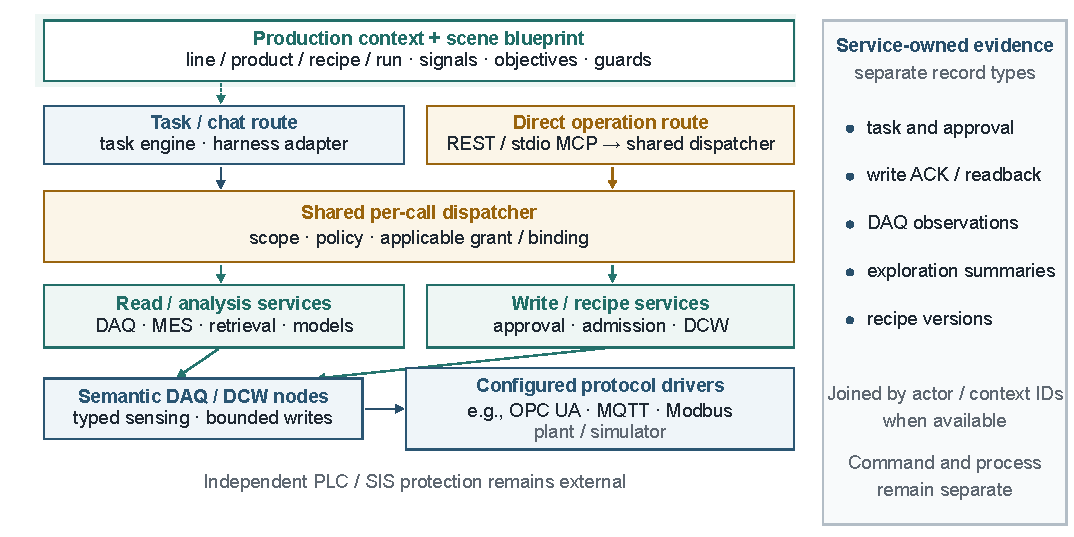
\includegraphics[width=\textwidth]{resources/fig-architecture-2026-9pt.pdf}
\caption{AgentWorkShop architecture and record ownership. Task/chat calls pass
through collaboration and a registered harness, whereas direct REST/stdio MCP
calls enter the shared dispatcher. Scene configuration and production context
inform task execution; operation handlers apply current route checks. Semantic
I/O resolves through configured drivers, while each service retains its own
records. Independent PLC/SIS protection remains external.}
\label{fig:arch}
\end{figure*}
\section{System Design}
\label{sec:design}
AgentWorkShop is designed for industrial tasks whose agents, production
contexts, interfaces, and process signals vary between deployments. Its
architecture organizes these variations around shared task and operation
services, checks each proposed operation against the active production
context before device routing, and retains route-specific evidence that
distinguishes a command receipt from a measured process response.

\subsection{Design Rationale and Requirements}
\label{sec:principles}
Five requirements---scene variability, harness variability, operation
authority, outcome observability, and extensibility---organize six design
rules (D1--D6). These are deployment constraints drawn from the target
workflows. D1 stores scene settings as versioned data;
D2 provides registered harness, tool, and driver interfaces; D3 separates
proposal from execution; D4 treats the tool catalog as discovery rather than
permission; D5 routes actuator writes through the common DCW admission point;
and D6 retains evidence by operation.

The requirements trace to implementation as follows.
Scene variability maps to D1, scene blueprints, and context resolution;
harness variability and extensibility map to D2, the registered harness and
driver interfaces; operation authority maps to D3--D5, the shared dispatcher,
grants, bindings, and write admission; outcome observability maps to D6,
route-specific receipts, and observations. R13 exercises two scene-specific
protocol and data paths; R20 exercises the configured task-to-device path
through one registered harness, synthetic approvals, and route-specific
records. Section~\ref{sec:eval} reports the experimental scope and evidence
limits. AgentWorkShop supplies task and operation services; agent strategy
and independent process protection remain outside this design.

\subsection{Layered Architecture}
\label{sec:layers}
\label{sec:arch}
Fig.~\ref{fig:arch} maps the reference implementation onto six bands and
their route-specific evidence records. The access band exposes command-line,
web, SDK, REST, MCP, and A2A entry surfaces. Task and chat routes enter the
collaboration band, which contains workspaces, channels, task queues, shared
memory, mailboxes, task templates, and harness adapters. A direct REST
tool-invocation route can call the shared operation dispatcher without
creating a task or invoking a harness; MCP also includes separate management
and task operations. The governance band projects an operation catalog and
checks each invocation. The context band assembles bound-line and active-run
information for prompt grounding, while operation handlers resolve the live
state relevant to their route. The service band provides acquisition, write
control, analysis, retrieval, and optional model services. The field-I/O band
resolves semantic nodes to built-in or plugin drivers for a plant or
simulator.

Each band has a distinct responsibility. Task/chat routes enter the task
runtime; direct operation routes enter the dispatcher; and both use shared
operation checks where applicable. A harness adapter supplies
agent-specific interaction on task paths, semantic nodes hide protocol
details from operations, and the driver registry provides the device-facing
extension point. Owning services retain task, command, observation, and
version records separately and link them to available actor and production
context. No single status conflates these outcomes.

\subsection{Cross-Module Execution Flow}
\label{sec:executionflow}
Fig.~\ref{fig:runtime} summarizes a task turn from entry through operation
execution, with route-specific evidence retained by owning services. Registered
harness adapters receive a scoped tool catalog during setup and supported
registry refreshes; the runtime assembles prompt-time production context for
each agent turn. This context is grounding information, not a task-pinned
transaction. For each returned tool call, the shared dispatcher rechecks
invocation scope and channel policy and, for industrial operations, current
grant and binding conditions before handler selection. The selected handler
then applies route-specific guards, active-run checks, approval
revalidation, and device-I/O steps as applicable. Command receipts and later
process observations remain distinct records.

For an industrial operation $u$ by agent $a$ in channel $c$, define the
shared dispatch condition as
\begin{equation}
\mathcal{A}(a,c,u)=S(a,c,u)\land P(c,u)\land G(a,u)\land B(a,u),
\label{eq:dispatch-contract}
\end{equation}
where $S$, $P$, $G$, and $B$ denote invocation scope, current channel policy,
runtime grant, and agent binding/resource ownership, as applicable to the
operation. The policy term includes
the applicable channel tool selection, profile, and duty-separation checks.
This condition is necessary for handler selection, not sufficient for
actuation: the selected route applies its own guards and approval, then
rechecks authority and applicable limits before dispatch.

Fig.~\ref{fig:execution} gives reference pseudocode for the registered-harness
task path, not one literal orchestrator function. Direct REST tool invocation
bypasses the task runtime and harness but enters the same shared dispatcher.
Route-specific timing, approval, and evidence rules are detailed in
Section~\ref{sec:modules}.

\begin{figure*}[!t]
\centering
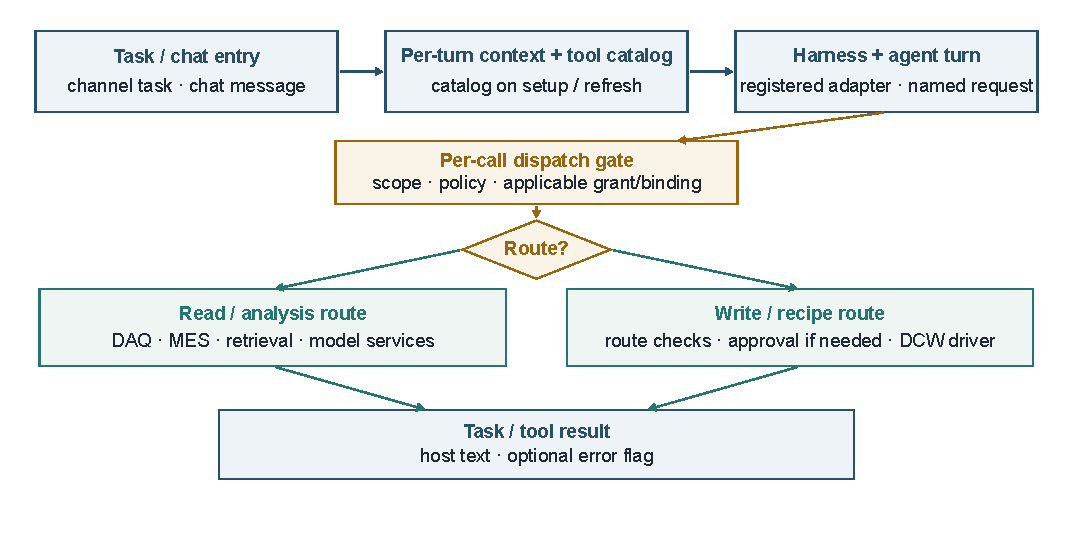
\includegraphics[width=\textwidth]{resources/fig-runtime-2026-9pt.pdf}
\caption{Registered-harness task execution in AgentWorkShop. The direct
REST tool-invocation route is outside this flow and enters the shared dispatcher
without a task or harness. The registered harness
uses a scoped catalog provisioned at setup and supported registry refreshes;
the runtime assembles prompt context per agent turn. The dispatcher checks
each returned call for scope, channel policy, and applicable grant and binding
conditions before handler selection. Route handlers resolve active-run and
approval-dependent state as applicable. The shared tool result contains host
text and an optional error flag; route records remain with owning services.
Prompt context is not a transactional authorization token. Dispatch-gate
errors return before handler execution, whereas route handlers may read state
before refusing a write. Durable denial auditing is selective. Receipts and
later observations remain distinct.}
\label{fig:runtime}
\end{figure*}

\begin{figure}[!t]
\centering
\begin{algorithmic}[1]
\Require task $q$, channel $c$, bound agent $a$, registered scoped catalog $T$
\Ensure task result; any retained evidence remains with its owning service
\State $x_t \gets \Call{ResolvePromptContext}{c,q}$
\State $m \gets \Call{RetrieveMemory}{q}$
\State $p \gets \Call{AssemblePrompt}{q,x_t,m}$
\State $h \gets \Call{InvokeRegisteredHarness}{a,p,T}$
\ForAll{tool request $u$ returned by $h$}
  \State $g \gets \Call{CheckScopeAndChannelPolicy}{a,c,u}$
  \If{\textbf{not} $g$}
    \State \Call{ReturnToolError}{h,u}; \textbf{continue}
  \EndIf
  \If{$u$ is an industrial operation}
    \State $v \gets \Call{CheckGrantBindingOwnership}{a,u}$
    \If{\textbf{not} $v$}
      \State \Call{ReturnToolError}{h,u}; \textbf{continue}
    \EndIf
  \EndIf
  \State $k \gets \Call{SelectHandler}{u}$
  \State $r \gets \Call{ExecuteRouteHandler}{k,a,c,u}$
  \Comment{handler resolves live state and may persist route-specific records}
  \State \Call{ReturnDeclaredToolResult}{h,r}
\EndFor
\State \Return task state and tool results
\end{algorithmic}
\caption{Reference pseudocode for the registered-harness task path.
Direct operation invocation is not shown. Evidence persistence is
route-specific and remains with the owning service; the shared tool result
does not carry a generic evidence envelope.}
\label{fig:execution}
\end{figure}

\section{Module Functions and Integration}
\label{sec:modules}
The architecture in Fig.~\ref{fig:arch} is implemented as cooperating
modules rather than a single monolithic agent. Shared interfaces connect
task execution to configuration, industrial services, protocol drivers, and
route-specific evidence. This section describes those responsibilities and
the checks that preserve their boundaries.

The implementation scope is broader than the evaluated scope. R20 exercises
the registered OMP task path, recipe-trial operation, two configured
signal/protocol mappings, synthetic approval, readback, and a run-tagged probe.
The separate regression run covers scope and grants, approval denial and
expiry, post-approval revalidation, node limits, and role-specific tool
exposure. Direct tool invocation, alternate harnesses, the normal online DAQ
backend, and physical equipment are not evaluated here.

The extension contracts expose the data passed at each boundary. A harness
call is normalized as \texttt{HostToolCall(toolName, arguments)} and returns
\texttt{HostToolResult(text, isError)}. A DCW driver accepts an engineering
value, tolerance, range, and driver configuration; its result separates write
status, raw value, readback, and acknowledgment grade (readback-verified,
transport-ack, or unverified). Each DAQ sample stores its node, timestamp,
value, and state, with optional line, product, recipe, and run IDs. A write
anchor records line/node, prior and requested values, source, actor, time, and
optional run/task/approval IDs; recipe definitions retain separate versions.
These fields keep tool errors, device receipts, observations, and production
lineage inspectable as separate records.

\subsection{Task Runtime and Harness Adapters}
Task and chat access surfaces create or join a workspace channel, where the
task engine manages members, task queues, shared memory, and execution
templates. A direct REST tool-invocation endpoint can enter the shared
dispatcher without creating a task or invoking a harness; the stdio MCP
operation bridge uses this route, while other MCP operations expose management
and task services.
The harness registry instantiates an adapter behind a common agent interface;
the prompt builder combines the task with the active scene brief, industrial
context, channel profile, agent binding, and retrieved memory. Tool calls
return to the shared dispatcher regardless of which registered harness
produced them. The registry is an extension point; the experiments do not
establish portability across harnesses. Industrial context is assembled for
each agent turn rather than pinned for the task lifetime. Operation handlers
check current route-specific state at invocation; recipe writes recheck the
binding, authorization, and active run after any human-approval wait. The
implementation does not compare the complete prompt-time
line--product--recipe--run snapshot with a task-pinned context version, so the
prompt snapshot is grounding information, not a transactional authorization
token.

\subsection{Production Context and Configuration}
Scene blueprints describe devices, signal maps, objectives, and process
guards. A task resolves these definitions against its active
line--product--recipe--run context. The channel profile selects the available
capability family, the tool policy narrows the operation catalog, and the
agent binding scopes the nodes, controls, and recipe operations available to
that member. These filters can restrict one another but cannot broaden the
underlying device range. The dispatcher re-reads policy at execution, so a
cached catalog does not retain authority after a grant or policy change. The
prompt builder assembles the agent's available bound-line and active-run
context on each turn; it does not pin the complete context tuple to the task.
Specific production snapshot, trial, and MPC routes, together with Hybrid Twin
training submissions, resolve and validate a versioned \texttt{SceneContract}
at operation time. The Twin physics-specification draft route can instead
accept a caller-supplied scene description; SceneContract enforcement is
therefore route-specific and does not validate or pin all prompt context.

\subsection{Acquisition, Analysis, and Modeling Services}
Semantic DAQ nodes expose typed values, engineering units, ranges, and
sampling settings while hiding protocol-specific reads. A per-node DAQ
runtime schedules acquisition and stores timestamped observations; the
gateway aggregates node pipelines. MES-facing operations provide the
configured production-data path. Analysis and retrieval services consume
these records, while optional model, training, optimization, and digital-twin
services are invoked through their registered operation handlers. These
services complement the agent workflow; AgentWorkShop does not prescribe a
single optimization strategy.

\subsection{Semantic I/O and Actuation}
The driver registry resolves a semantic node to a built-in or plugin driver.
DAQ handlers use the node's acquisition interface; DCW handlers route a
write or readback through the controller and the configured protocol driver.
This separation lets recipes and agents refer to semantic controls without
embedding Modbus, OPC UA, MQTT, HTTP, or MES transport details in their
operation arguments. The supported driver mappings are implementation
interfaces; only the mappings and workflows enumerated in Section~\ref{sec:eval}
are experimentally exercised.

\subsection{Shared Dispatch and Write Admission}
\label{sec:governed}
Every named operation passes the dispatcher. Its ordered checks validate
invocation scope and current channel policy (tool selection, profile, and
applicable duty separation), then the agent's binding and runtime grant and
ownership of referenced resources.
A refusal returns the excluding condition. Denial persistence is selective:
grant denials and selected resource-reference denials have explicit audit
paths, whereas scope and channel-policy denials are not uniformly retained as
durable audit events. A catalog entry therefore describes availability but
does not authorize execution. Handlers
for operations that require manual approval suspend for a decision, then
revalidate authority and active limits before dispatch.

All actuator writes converge on the DCW admission point. For an online node
write, the admissible interval is
\begin{equation}
\mathcal{I}^{\mathrm{online}}_n(t)=\mathcal{H}_n\cap\mathcal{B}_n
\cap\mathcal{P}_n(t)\cap\mathcal{R}_n(t),
\label{eq:admission}
\end{equation}
where $\mathcal{H}_n$ is the hard engineering range and $\mathcal{B}_n$,
$\mathcal{P}_n$, and $\mathcal{R}_n$ are the baseline, active-product, and
active-recipe limits. Missing optional limits impose no restriction, whereas
an empty intersection rejects the request and identifies the excluding
layer. Recipe dispatch applies the hard, baseline, and product limits to the
replacement recipe rather than intersecting with the previous recipe window.
The actuator path also enforces step, interval, and hold-window checks.
These admission rules constrain commands; process objectives and coupled
variable guards are assessed from later observations. The framework does
not replace independent PLC or safety-instrumented protection.

\subsection{Integrated Operation and Route-Specific Evidence}
\label{sec:tasklifecycle}
A recipe trial illustrates how the modules cooperate. The task runtime
delivers a named \texttt{recipe\_trial} call from the agent harness; the
dispatcher checks the agent's recipe binding and execution scope; the recipe
handler checks the active run, candidate parameters, and route timing; and a
manual binding requests approval before the DCW controller sends the batch
through its driver. The handler returns a per-parameter receipt. The caller
then obtains DAQ observations and can request a separate update, apply, or
rollback operation. A trial receipt confirms command handling; it does not
by itself establish process attainment or persist a new recipe version.

The routes retain different records because they answer different
questions. A driver acknowledgment reports command evidence; DAQ reports a
process observation; an exploration summary records a bounded probe; and a
recipe version records a saved definition. Their relation through actor and
production context allows an execution to be inspected without treating
these outcomes as interchangeable.

\subsection{Route-Specific Lifecycles and Evidence}
\label{sec:routes}
\label{sec:mech}
\label{sec:objective}
\label{sec:nodeexec}
\label{sec:ack}

\paragraph{Timing and approval}
Timing guards are route-specific. Online node writes enforce an effective
minimum spacing of 60\,s. Recipe dispatch uses a per-recipe interval anchored
to approval, while trials also use a configurable per-line cadence (default
300\,s). The recipe interval can refuse a proposal before an approval request
is created. Checks occur at proposal or execution according to the operation,
and experiment-specific pacing overrides are reported with the corresponding
results.

Manual bindings create an approval request containing the actor, node or
recipe, candidate values, applicable limits, expiry, and parameter bases.
The default wait expires after 180\,s and refuses execution. After approval,
the executor rechecks authorization and active limits to account for context
changes during the wait. For \texttt{recipe\_apply}, a changed definition
requires a new proposal; an unchanged approval dispatches a copy of the
approved parameter snapshot. A line-level recipe mode defaults to manual;
changing it to automatic requires administrator confirmation. The approval
record authorizes a workflow action and does not replace process protection.

\begin{figure*}[!t]
\centering
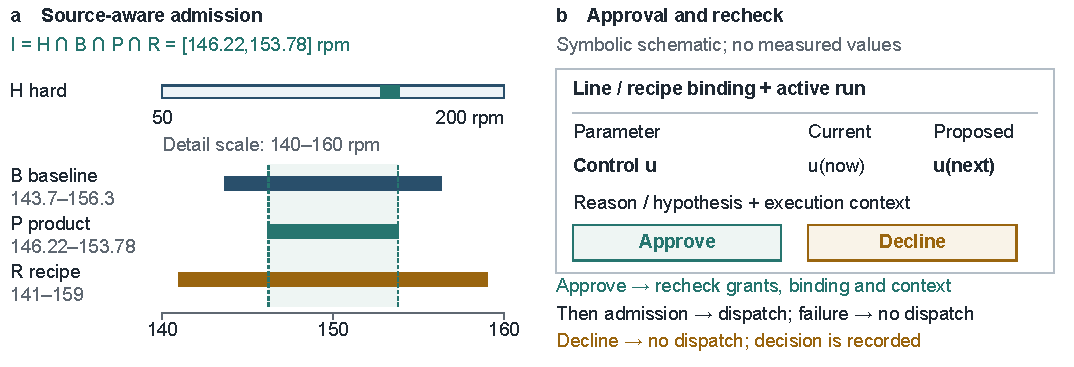
\includegraphics[width=\textwidth]{resources/fig-admission-hitl-2026.pdf}
\caption{Admission and approval boundaries. (a) Illustrative archived RPM
configuration (not part of R20):
online node interventions use the four-layer value interval of
Eq.~(\ref{eq:admission}),
whereas recipe dispatch omits the prior recipe window. (b) Symbolic human
approval binds a proposed action and authority fields; execution checks run
again after approval, which does not reserve equipment state.}
\label{fig:hitl}
\end{figure*}

\paragraph{Node probe}
The bounded \texttt{optimization\_explore} route is exposed to the AML
optimization profile. It validates a bound control and DAQ scope, captures a
baseline, routes a bounded write through DCW, and stores a later target window
as a separate exploration summary. Its timing and approval behavior is
route-specific; R20 does not exercise this route.

\paragraph{Recipe operations}
\texttt{recipe\_trial} checks the bound recipe and active run, then dispatches
candidate overrides as a batch with per-parameter verification. The caller
subsequently queries DAQ and may save a definition with
\texttt{recipe\_update}, restore one with \texttt{recipe\_rollback}, or apply
a version with \texttt{recipe\_apply}. A trial does not save or apply a
version, and endpoint verification is not a process-response measurement.
Public direct-node control is closed; bounded probes and recipe operations are
the configured write surfaces.

\paragraph{Command verification}
Command confirmation and process response answer different questions. A
driver ACK is graded as \texttt{readback-verified}, \texttt{transport-ack},
or \texttt{unverified}; a matching endpoint read supports the first grade,
whereas transport or MES application confirmation supports the second.
Recipe-batch verification is \texttt{verified}, \texttt{unverified}, or
\texttt{failed}. If readback is absent or mismatched, up to three reads are
attempted 2\,s apart. Initial ACKs, final ACKs, and per-parameter verdicts are
retained separately. A readback-verified setpoint does not establish target
attainment.

\paragraph{Observation, verdict, and compensation}
Recipe-path observation follows batch dispatch, and saving a definition,
applying it, and observing process response remain separate operations. An
open node record can request rollback after repeated breaches; missing samples
do not count as breaches. Caller verdicts and compensation remain separate
from the observation and subject to admission checks.
\label{sec:agentloop}


\FloatBarrier
\section{Experimental Evaluation}
\label{sec:eval}
The evaluation asks whether one registered-harness path can execute bounded
tasks across two simulator scenes with different signal and protocol mappings
while retaining a checkable task-to-approval-to-receipt-to-sample trace. R20 is
the primary result: six sequential tasks through one registered harness, three
per scene on one simulator instance per scene. It demonstrates this configured
software path, not configuration-reuse benefit or process attainment. R13 is
secondary exploratory protocol and data-path evidence whose exact runtime
source was not pinned. All experiments use repository simulators. An anonymous
evidence archive is supplied as Supplementary File~S1; its trace matrix and
run records support the R20 checks reported below.

\subsection{Evidence Units and Experimental Procedure}
\label{sec:testbed}
\label{sec:procedure}
R20 uses the registered \texttt{omp} harness in cast-film and annealing scenes,
with three sequential task executions per scene on one simulator instance per
scene. R13 uses configured protocol and data paths in the same two simulator
scenes. Earlier experiments are retained separately in Supplementary File~S1
and are not pooled with these results.

\subsection{Registered-Harness Process Path (R20)}
\label{sec:harness-e2e}
R20 ran the local v0.8.0 working-tree application with the registered
\texttt{omp} adapter and GLM-5.3-Flash. Supplementary File~S1 contains the
recorded base revisions, working-tree patches, dependency lockfiles, prompt
assets, and run logs. This is a source-reconstruction kit rather than an
immutable release, and the external model service does not guarantee
deterministic replay. Each of six sequential executions created a separate
line, product, recipe, run, channel, agent, and task context. Three executions
shared one simulator instance per scene. Cast film used OPC UA for screw-speed
control and MQTT for thickness; annealing used Modbus TCP for both the zone-3
setpoint and strip-temperature probe. The model received a live control read,
process measurement, and target band, then selected one value from the
scenario-defined prevalidated set (125/130/135 rpm or 735/740/745~$^{\circ}$C)
for a bounded \texttt{recipe\_trial}; this was a constrained choice, not an
unrestricted optimization search. A synthetic administrator approved each
proposal. Each route log contains one trial and a 1/1 verified device receipt.

After verifying the route ACK and returned trial result, the runner initiated
a 20-s delay, then probed, ingested, and queried one value per task under the
active-run tag through the isolated SQLite time-series fallback. The runner
checked task state after the sample query; all six task records were then
\texttt{COMPLETED}. The runner reported 76 passing checks and no failures, and
the separate trace audit found a complete task-to-sample record in all six
executions: each had a matching approval ID, one readback-verified trial
receipt, and one query result whose run ID and value matched the active run and
explicit probe. The task-completion timestamp was not retained, so no
task-completion-to-sample interval can be computed. Table~\ref{tab:q8} labels
Film-1--3 map to \texttt{cast-film-r1--r3}, and Anneal-1--3 to
\texttt{annealing-r1--r3}; full identifiers and per-record checks are listed
in \texttt{R20-TRACE-MATRIX.csv} in S1.

Table~\ref{tab:q8} reports the pre-task process value, selected setting, and
run-tagged sample for each execution. All six samples remained outside target.
The experiment verifies the bounded harness-to-simulator execution and record
path, not process attainment or convergence. Task completion denotes a
completed software workflow, not satisfaction of the manufacturing objective.
A single probe is not a response trajectory, and the SQLite fallback does not
test the normal online DAQ backend. R20 also does not isolate
profile/binding reuse or establish cross-harness portability.

\begin{table}[!t]
\centering
\caption{Constrained model selections and simulator measurements. The control
is screw speed for cast film and the zone-3 furnace setpoint for annealing.
Each row reports one run-tagged probe after a 20-s delay from verified route
readback. All six samples are outside target; executions are sequential within
each scene.}
\label{tab:q8}
\footnotesize
\setlength{\tabcolsep}{2.5pt}
\begin{tabularx}{\columnwidth}{@{}lXcX@{}}
\toprule
Case & Pre-task value / target band & Control: start$\to$trial & Sample \\
\midrule
Film-1 & $55.82/48$--$52~\mu$m & $120\to125$~rpm & $45.69~\mu$m \\
Film-2 & $45.69/48$--$52~\mu$m & $120\to130$~rpm & $46.69~\mu$m \\
Film-3 & $46.69/48$--$52~\mu$m & $120\to125$~rpm & $45.69~\mu$m \\
Anneal-1 & $675.40/700$--$760~^{\circ}$C & $730\to745$~$^{\circ}$C & $679.60~^{\circ}$C \\
Anneal-2 & $678.30/700$--$760~^{\circ}$C & $730\to745$~$^{\circ}$C & $677.70~^{\circ}$C \\
Anneal-3 & $676.90/700$--$760~^{\circ}$C & $730\to745$~$^{\circ}$C & $678.10~^{\circ}$C \\
\bottomrule
\end{tabularx}
\end{table}

\subsection{Software Contract Checks}
A separate regression run on the local v0.8.0 working tree records 65 passing
software tests across eight suites and no failures. Denied or expired
approvals, changed recipe or limit state after approval, and invalid node
values are refused before driver actuation; unchanged approved state dispatches
through the mock driver and readback. The suites also cover tool scope, grants,
and role-specific exposure. These checks use temporary or mock state and are
separate from R20's 76 runner checks; they do not represent process trials or
test missing/mismatched DAQ run tags in the end-to-end path.

\subsection{Exploratory Protocol and Data Path (R13)}
\label{sec:crossscene}
The R13 application report describes five protocol-family read probes (OPC UA,
MQTT, Modbus TCP, Modbus RTU over TCP, and HTTP/REST) and bounded writes with
matching readbacks in two simulator scenes. Six sequential 120-s windows per
scene at 1-s sampling produced lineage-verified datasets with 658 cast-film
rows and 655 annealing rows. The rows are overlapping time-window samples, not
independent process replications. The exact runtime source was not recorded. R13 is
used only as exploratory protocol and data-lineage evidence; its archived gate
outputs and run-boundary audit are documented in the reproducibility
supplement and do not support the primary registered-harness result.

Earlier protocol, admission-ablation, controller, deployment, and scripted
recipe records in S1 use older versions or interfaces. They are not pooled
with R13 or R20, used as matched strategy comparisons, or relied on for the
current integration claims.

\section{Discussion}
\label{sec:limits}
R20 demonstrates the bounded registered-harness path across the two tested
simulator scenes: tasks completed with synthetic approval and verified
readback, and all six records passed the task-to-approval-to-receipt-to-sample
link checks. No post-trial sample reached its target band. The 20-s sample
delay began after receipt/readback verification; the runner checked task state
after the sample query, and no task-completion-to-sample interval is retained.
R13 separately contributes exploratory protocol and data-lineage evidence.
Neither run establishes process-control efficacy.

R20 uses one simulator instance per scene and does not establish independent
replication, convergence, or quality improvement. Its single post-trial
sample per execution is not a response trajectory or a
task-completion-to-sample latency measurement. Controlled profile/binding
adaptation, cross-harness portability, normal online DAQ backend behavior, and
physical transfer remain untested. The synthetic approval records do not
measure operator effectiveness
\cite{parasuramanmanzey2010complacency,parasuraman2000model,bainbridge1983ironies};
restricted tool access does not establish deployment security
\cite{greshake2023injection,liu2024pinjection,iec62443-3-3} or replace
independently engineered PLC/SIS protection \cite{iec61511}.

The next evaluation should use an immutable build, independent simulator
replications, a controlled configuration-change or reuse test, normal online
DAQ, and physical-plant trials. These experiments would test whether the
implemented trace contract improves integration practice beyond the two
configured paths reported here.

\section{Conclusion}
\label{sec:conclusion}
AgentWorkShop provides a reference implementation that joins collaborative
harnesses, production context, operation checks, semantic I/O, and
route-specific records. R20 demonstrates a task-to-sample trace in two
simulator scenes, with complete linkage checks for six executions and all six
post-trial samples outside target. R13 supplies secondary protocol and
data-path evidence. The results establish behavior of the tested software
paths, not process-control efficacy or portability.


% TII's anonymous-review checklist requires acknowledgments to be omitted.
% Restore the separate AI disclosure after the review stage; see the author note.

\bibliographystyle{IEEEtran}
% Keep IEEEtran's default bibliography size and leading.
\bibliography{resources/refs}

\end{document}
